\begin{infocard}{Gráficas de ecuaciones cuadráticas}
    \begin{figure}[H]
        \centering
        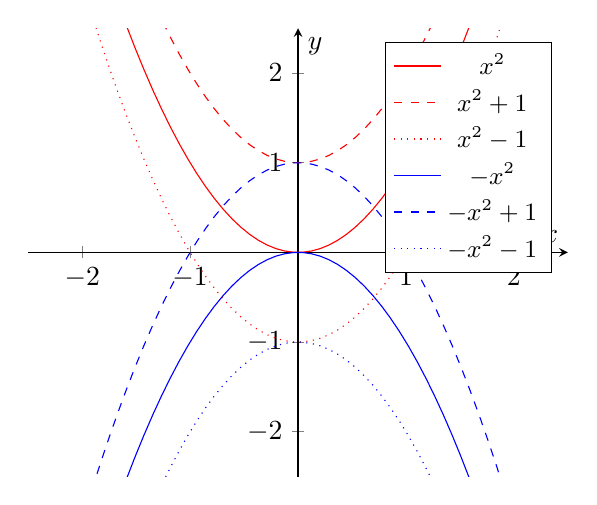
\begin{tikzpicture}
            \begin{axis}
                [
                    legend style={ at={(0.5,1)}, font=\small},
                    legend pos=north east,
                    %legend columns=3,
                    axis lines = center,
                    domain=-2:2,
                    xlabel=$x$,
                    xmin=-2.5,
                    xmax=2.5,
                    xtick={-2,-1,0,1,2},
                    ylabel=$y$,
                    ymin=-2.5,
                    ymax=2.5,
                    ytick={-2,-1,0,1,2},
                    samples=50,
                ]
                \addplot [red] {x^2};
                \addplot [red,dashed] {x^2+1};
                \addplot [red,dotted] {x^2-1};
                \addplot [blue] {-x^2};
                \addplot [blue,dashed] {-x^2+1};
                \addplot [blue,dotted] {-x^2-1};
                \legend{$x^2$,$x^2+1$,$x^2-1$,$-x^2$,$-x^2+1$,$-x^2-1$}
            \end{axis}
        \end{tikzpicture}
        \caption{Grafica de $x^2$ (rojo), su negarivo $-x^2$ (azul) y su variación en el término independiente (líneas punteadas).}
        \label{fig:analytical}
    \end{figure}
\end{infocard}

%----------------------------------------------------------------------------------------

